%%%%%%%%%%%%%%%%%%%%%%%%%%%%%%%%%%%%%%%%%
% Jacobs Landscape Poster
% LaTeX Template
% Version 1.1 (14/06/14)
%
% Created by:
% Computational Physics and Biophysics Group, Jacobs University
% https://teamwork.jacobs-university.de:8443/confluence/display/CoPandBiG/LaTeX+Poster
% 
% Further modified by:
% Nathaniel Johnston (nathaniel@njohnston.ca)
%
% This template has been downloaded from:
% http://www.LaTeXTemplates.com
%
% License:
% CC BY-NC-SA 3.0 (http://creativecommons.org/licenses/by-nc-sa/3.0/)
%
%%%%%%%%%%%%%%%%%%%%%%%%%%%%%%%%%%%%%%%%%

\documentclass[final]{beamer}

\usepackage[scale=1.2]{beamerposter} % Use the beamerposter package for laying out the poster

\usetheme{confposter} % Use the confposter theme supplied with this template
%\usetheme{Madrid} % Use the confposter theme supplied with this template

\makeatletter
\providecommand*{\input@path}{}
\g@addto@macro\input@path{{fig/}{../figures/}}
\makeatother

\usepackage{graphicx}
\graphicspath{{fig/}{../figures/}}

\usepackage{xcolor}
\definecolor{hdcolor}{HTML}{c81f32}
\definecolor{hdcolor2}{HTML}{f94a5e}
\definecolor{hdcolordark}{HTML}{4f0c12}
\definecolor{jblue}{HTML}{c81f32}

\usepackage{siunitx}
\usepackage{enumitem}
\usepackage{booktabs} % professional table layout
\usepackage{tikz}
\usetikzlibrary{positioning}

\newcommand*\circled[2]{\tikz[baseline=(char.base)]{%
            \node[shape=circle,fill=#2,draw,inner sep=2pt] (char) {#1};}}
\newcommand*\cwhite[1]{\tikz[baseline=(char.base)]{%
            \node[shape=circle,fill=white,draw,inner sep=2pt] (char) {#1};}}
\newcommand*\cplus{\circled{\small$+$}{green}}
\newcommand*\cminus{\circled{\small$-$}{red}}

% Many more colors are available for use in beamerthemeconfposter.sty
\setbeamercolor{palette primary}   {fg=black,bg=white}
\setbeamercolor{palette secondary} {fg=black,bg=white}
\setbeamercolor{palette tertiary}  {bg=jblue,fg=white}
\setbeamercolor{palette quaternary}{fg=black,bg=white}
\setbeamercolor{structure}{fg=jblue}
\setbeamercolor{titlelike}         {bg=jblue,fg=white}
\setbeamercolor{frametitle}        {bg=jblue!10,fg=jblue}
\setbeamercolor{cboxb}{fg=black,bg=jblue}
\setbeamercolor{cboxr}{fg=black,bg=red}
% set colors for itemize/enumerate
\setbeamercolor{item}{fg=black}
\setbeamercolor{item projected}{fg=black,bg=gray}
% set colors for blocks
\setbeamercolor{block title}{fg=black,bg=white}
\setbeamercolor{block body}{fg=black,bg=white}
% set colors for alerted blocks (blocks with frame)
\setbeamercolor{block alerted title}{fg=white,bg=jblue}
\setbeamercolor{block alerted body}{fg=black,bg=jblue!10}

%-----------------------------------------------------------
% Define the column widths and overall poster size
% To set effective sepwid, onecolwid and twocolwid values, first choose how many columns you want and how much separation you want between columns
% In this template, the separation width chosen is 0.024 of the paper width and a 4-column layout
% onecolwid should therefore be (1-(# of columns+1)*sepwid)/# of columns e.g. (1-(4+1)*0.024)/4 = 0.22
% Set twocolwid to be (2*onecolwid)+sepwid = 0.464
% Set threecolwid to be (3*onecolwid)+2*sepwid = 0.708

\newlength{\sepwid}
\newlength{\onecolwid}
\newlength{\twocolwid}
\newlength{\threecolwid}
\setlength{\paperwidth}{48in} % A0 width: 46.8in
\setlength{\paperheight}{36in} % A0 height: 33.1in
\setlength{\sepwid}{0.024\paperwidth} % Separation width (white space) between columns
\setlength{\onecolwid}{0.22\paperwidth} % Width of one column
\setlength{\twocolwid}{0.464\paperwidth} % Width of two columns
\setlength{\threecolwid}{0.708\paperwidth} % Width of three columns
\setlength{\topmargin}{-0.5in} % Reduce the top margin size
%-----------------------------------------------------------

\usepackage{booktabs} % Top and bottom rules for tables

%----------------------------------------------------------------------------------------
%	TITLE SECTION 
%----------------------------------------------------------------------------------------

\title{Brain Tumor Segmentation with Random Forest and U-Net} % Poster title

\author{Shuhan Xiao and Alexander Kugele} % Author(s)

\institute{Heidelberg University} % Institution(s)

%----------------------------------------------------------------------------------------

\begin{document}

\addtobeamertemplate{block end}{}{\vspace*{2ex}} % White space under blocks
\addtobeamertemplate{block alerted end}{}{\vspace*{2ex}} % White space under highlighted (alert) blocks

\setlength{\belowcaptionskip}{2ex} % White space under figures
\setlength\belowdisplayshortskip{2ex} % White space under equations

\begin{frame}[t] % The whole poster is enclosed in one beamer frame

\begin{columns}[t] % The whole poster consists of three major columns, the second of which is split into two columns twice - the [t] option aligns each column's content to the top

\begin{column}{\sepwid}\end{column} % Empty spacer column

\begin{column}{\onecolwid} % The first column

\begin{block}{Motivation}
\begin{itemize}[label={}]
\item Brain tumors need immediate treatment
\item Even experts can not segment perfectly
\item Takes time to go through a complete MR scan
\end{itemize}
Efficiently segmenting tumors automatically improves treatment planing
\end{block}

\begin{alertblock}{Dataset}
\begin{itemize}[label={}]
\item 3D MR scans of 275 human brains
\item 4 scan types, T1, T1c, T2 and Flair
\item $\mathrm{depth}=155$, $\mathrm{height}=240$, $\mathrm{width}=240$
\item $\Rightarrow 170500$ images
\item 5 classes (we only use 2)
\item center-cropped to $80\%$ of their size
\end{itemize}
\begin{figure}
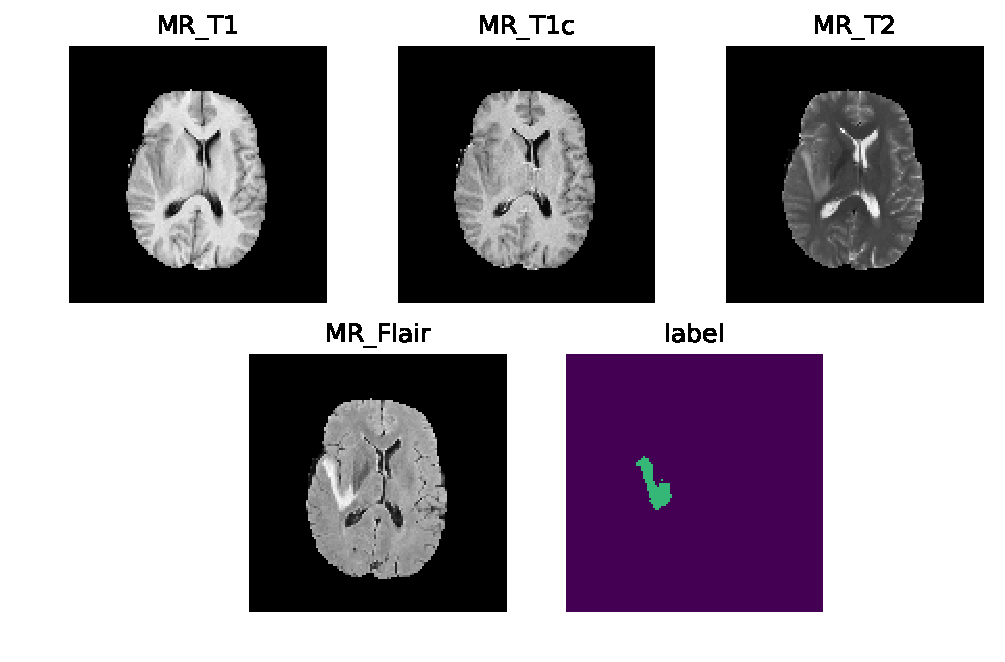
\includegraphics[width=0.9\linewidth]{scan_types_trans}
\end{figure}

\end{alertblock}

\begin{block}{Features}
\begin{itemize}[label={}]
\item Gaussian, LoG, Gaussian gradient
\item Hessian and structure tensor eigenvalues
\item equalized histogram
\item 29 features in total
\item 1k images + features $\approx \SI{30}{GB}$ of memory
\end{itemize}
\begin{figure}
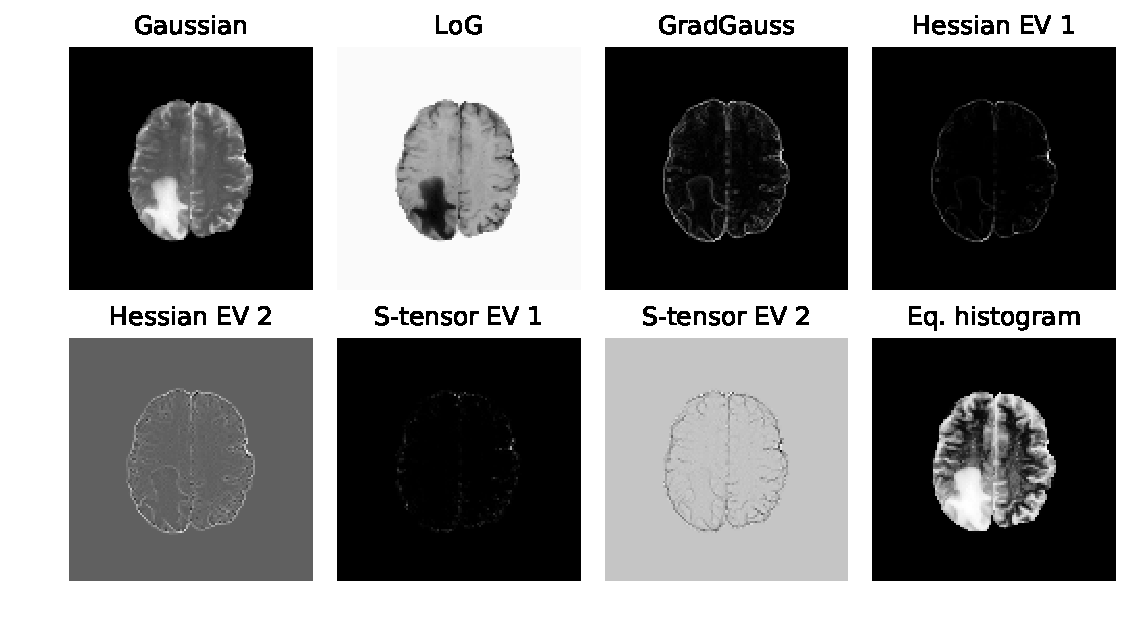
\includegraphics[width=0.97\textwidth]{features}
\end{figure}
\end{block}


\end{column} % End of the first column

\begin{column}{\sepwid}\end{column} % Empty spacer column

\begin{column}{\twocolwid} % Begin a column which is two columns wide (column 2)

\begin{columns}[t,totalwidth=\twocolwid] % Split up the two columns wide column

\begin{column}{\onecolwid}\vspace{-.6in} % The first column within column 2 (column 2.1)

\begin{alertblock}{Random Forest}
\begin{itemize}[label={}]
\item trained in batch-mode \cite{batchrf}
\item 100 estimators per batch, 3 batches of 1k images
\end{itemize}
Advantages and disadvantages
\begin{description}
\item[\cplus] Easier to understand
\item[\cplus] Rarely overfits
\item[\cplus] Single pixel training
\item[\cminus] No GPU training
\item[\cminus] No incremental training (for vanilla RF)
\item[\cminus] Features have to be hand-selected
\end{description}
\end{alertblock}


\end{column} % End of column 2.1

\begin{column}{\onecolwid}\vspace{-.6in} % The second column within column 2 (column 2.2)

\begin{block}{Methods}

\end{block}

\end{column} % End of column 2.2

\end{columns} % End of the split of column 2 - any content after this will now take up 2 columns width

\begin{alertblock}{Comparison}
\centering
	\begin{tabular}{lrrr}
	\toprule
	 & Dice [$\%$] & Sensitivity [$\%$] & Specificity [$\%$] \\
	\midrule
	Random Forest & $65.9$ & $77.1$ & $99.1$ \\
	U-Net & & & \\
	\bottomrule
	\end{tabular}
\end{alertblock}

%----------------------------------------------------------------------------------------

\begin{columns}[t,totalwidth=\twocolwid] % Split up the two columns wide column again

\begin{column}{\onecolwid} % The first column within column 2 (column 2.1)

\begin{block}{RF: Results}
\begin{itemize}[label={}]
\item training time $\approx \SI{13}{h}$
\item inference time $\approx \si{2-20}{s}$ per image
\item load time $\approx \si{310}{s}$
\item disk space $\approx \SI{15}{GB}$ (pickled)
\item memory space during inference $\approx \SI{20}{GB}$
\end{itemize}
\begin{figure}
\centering
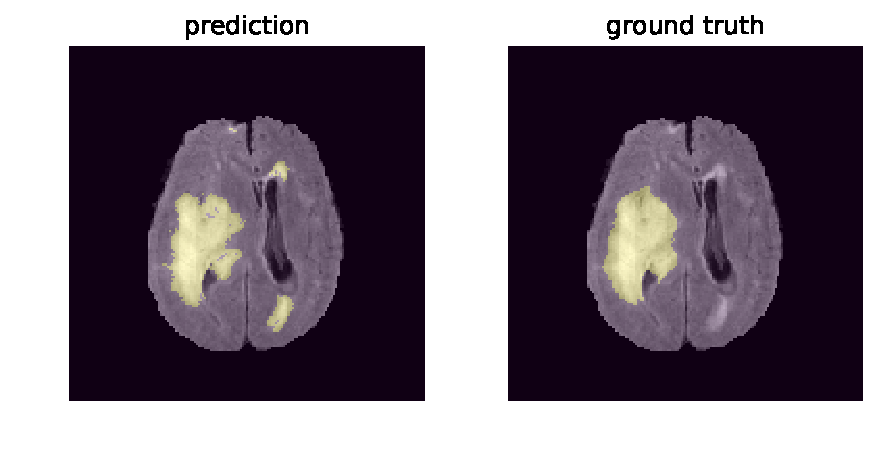
\includegraphics[width=0.9\linewidth]{rf_prediction_84}
\end{figure}
\end{block}

%----------------------------------------------------------------------------------------

\end{column} % End of column 2.1

\begin{column}{\onecolwid} % The second column within column 2 (column 2.2)

%----------------------------------------------------------------------------------------
%	RESULTS
%----------------------------------------------------------------------------------------

\begin{block}{Results}


\end{block}

%----------------------------------------------------------------------------------------

\end{column} % End of column 2.2

\end{columns} % End of the split of column 2

\end{column} % End of the second column

\begin{column}{\sepwid}\end{column} % Empty spacer column

\begin{column}{\onecolwid} % The third column

%----------------------------------------------------------------------------------------
%	CONCLUSION
%----------------------------------------------------------------------------------------

\begin{block}{Conclusion}

\end{block}

\begin{block}{Additional Information}

\end{block}

\begin{block}{References}

%\nocite{*} % Insert publications even if they are not cited in the poster
\small{\bibliographystyle{unsrt}
\bibliography{../biblio}\vspace{0.75in}}

\end{block}

%\setbeamercolor{block title}{fg=red,bg=white} % Change the block title color

\begin{block}{Acknowledgements}

\end{block}

%----------------------------------------------------------------------------------------
%	CONTACT INFORMATION
%----------------------------------------------------------------------------------------

%\setbeamercolor{block alerted title}{fg=black,bg=norange} % Change the alert block title colors
%\setbeamercolor{block alerted body}{fg=black,bg=white} % Change the alert block body colors

\begin{flushright}

\includegraphics[width=0.5\linewidth]{logo_hd.pdf}
\end{flushright}

%----------------------------------------------------------------------------------------

\end{column} % End of the third column

\end{columns} % End of all the columns in the poster

\end{frame} % End of the enclosing frame

\end{document}
